% ERA-Großpraktikum: Entwickleranleitung -- Module

\section{Module}

Diese Sektion führt in den Aufbau des Simulators ein und beschreibt detailliert
die einzelnen Funktionen der Module. Das Ziel dieser Sektion ist es, neue
Entwickler mit dem Aufbau unseres Codes vertraut zu machen, sodass diese in der
Lage sind, selbstständig Änderungen am Code vorzunehmen. \\
Zunächst wird ein Überblick über den Aufbau des Programms gegeben und
anschließend ausführlich auf die einzelnen Module eingegangen.

\subsection{Überblick}

Wir haben den Simulator in vier Module aufgeteilt, die jeweils unterschiedliche
Aufgaben bei der Simulation eines Befehlssatzes übernehmen.

Die \textbf{Architektur} ist für die Ausführung eines simulierten Assembler
Programms zuständig und implementiert die verfügbaren Befehlssätze (zum Stand
dieses Berichts \textit{RISCV}). Des Weiteren stellt das Architekturmodul
die Befehlssatz-spezifischen Fehler- und Hilfetexte zur Verfügung, die dem
Anwender im Endprodukt präsentiert werden. \\
Von der Idee geleitet, dass verschiedene Assembler Dialekte für den gleichen
Befehlssatz existieren, ist der \textbf{Parser} ein eigenes Modul, der für die
Übersetzung des Assembler Quelltextes zuständig ist. Der Parser übersetzt die
möglicherweise verschiedenen Assembler Dialekte in ein allgemeines Format (wir
sprechen dabei von einem \textit{Syntax Baum}), das anschließend von der Architektur
verarbeitet werden kann. \\
Die einzelnen Module werden vom \textbf{Core} verbunden. Der Core ist das
Herzstück des Simulators und regelt die Kommunikation zwischen allen anderen
Modulen. Insbesondere stellt er der Architektur eine Umgebung zur Verfügung, in
der diese arbeiten kann (Speicher, Register). Des Weiteren ist er für die
Verwaltung der verschiedenen Threads zuständig. \\
Die \textbf{GUI} (Graphical User Interface) implementiert die grafische
Oberfläche des Simulators. Sie ist bewusst abgekoppelt vom Rest der Module,
um auch durch andere Oberflächen (wie z.B. einer Kommandozeile) ausgetauscht
werden zu können. Die grafische Oberfläche leitet die Benutzereingaben an den
Core weiter, welcher dann wiederum die übrigen Module anspricht.

\subsection{Architektur}

\todo[inline]{
	* Syntax Tree \\
	* Factory \\
	* Architecture \\
	* Teilung common/riscv \\
	* ValidationResult \\
	* InstructionNode \\
}

Die Architektur (kurz: \textit{Arch}) kümmert sich um die Ausführung der
Assembler Programme und wurde vor dem Hintergrund entworfen, einen möglichst
Architektur-unabhängigen Simulator zu entwickeln. So stellt sie Klassen zur
Verfügung, mit der eine konkrete Architektur (wie z.B. RISC-V) umgesetzt
werden kann. Eine Architektur kann in \texttt{YAML} Konfigurationsdateien
beschrieben, und anschließend in das Programm geladen werden. \\
Da wir uns gegen die Ausführung von Maschinencode entschieden haben, bietet
die Architektur eine abstraktere Darstellung von Assembler Programmen in Form
eines Syntax Baums. Des Weiteren ist die Architektur für die Validierung einer
Instruktion zuständig, und stellt bei Fehlern entsprechende Nachrichten zur
Verfügung, die dem Nutzer helfen sollen, das Problem zu beheben.

\begin{figure}[H]
	\centering
	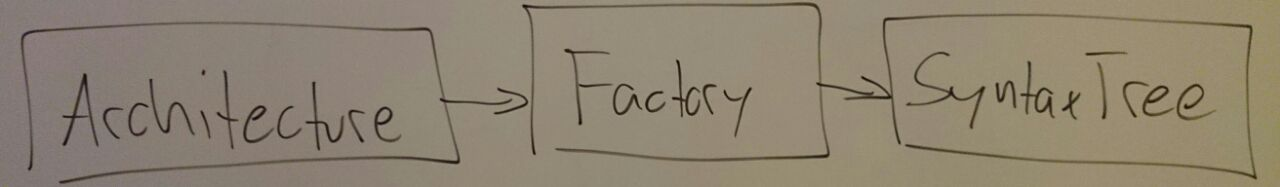
\includegraphics[width=\textwidth,keepaspectratio]{img/arch-overview.jpg}
	\caption{Schnittstelle Architektur Übersicht (sehr professionell)}
	\label{fig:arch-overview}
\end{figure}

Abbildung \ref{fig:arch-overview} zeigt eine Übersicht über die Schnittstelle zu den
anderen Modulen.
\todo[inline]{Mit dem Bild will ich das Zusammenspiel aus Architecture,
Factory und SyntaxTree zeigen. Da brauchen wir vielleicht ein besseres Diagramm ;)}

\subsubsection{Architecture Description Language}

Eine Architektur kann in \texttt{YAML} Dateien beschrieben werden.

\todo[inline]{@Peter}

\subsection{Parser}

\subsection{Core}

Beschreibung des Moduls + Schnittstellen zu anderen Modulen

\subsection{GUI}
